\documentclass[preprint, 11pt]{article}

\usepackage[T1]{fontenc}
\usepackage[utf8]{inputenc}
\usepackage[hmargin=0.9in, vmargin=1.25in]{geometry}
\usepackage[babel]{csquotes}
\usepackage{subfig}
\usepackage{graphicx}
\usepackage[colorlinks=true,citecolor=blue,urlcolor=blue]{hyperref}
\usepackage{caption}
\usepackage{amsmath}          % writing mathematical formulas
\usepackage{amsthm}           % writing mathematical theorems 
\usepackage{amssymb}          % writing mathematical symbols
\usepackage{bm, amsfonts}     % writing bold mathematical symbols
\usepackage{xcolor}
\usepackage{fixmath}
\usepackage{tikz}
\usepackage{bm}
\usepackage{makecell}
\usepackage{mathdots}
\usepackage{algpseudocode}
\usepackage{algorithm}

\newcommand{\W}{{\mathcal W}}
\newcommand{\A}{{\mathcal A}}
\newcommand{\bff}{{\bf f}}
\newcommand{\bfr}{{\bf r}}
\newcommand{\bfF}{{\bf F}}
\newcommand{\bfu}{{\bf u}}
\newcommand{\bfv}{{\bf v}}
\newcommand{\bfq}{{\bf q}}
\newcommand{\bfx}{{\bf x}}
\newcommand{\sgn}{{\rm sgn}}
\newcommand{\Rus}{{\rm Rus}}
\newcommand{\Roe}{{\rm Roe}}

%\newdefinition{rmk}{Remark}
\newtheorem{remark}{Remark}

\title{Numerical simulation and entropy dissipative cure of the 
  carbuncle instability for the shallow water circular hydraulic jump}

\author{
    David I. Ketcheson \and
    Manuel Quezada de Luna
}
\begin{document}

\maketitle

\begin{abstract}

\end{abstract}

\section{Introduction}

\subsection{The circular hydraulic jump}

\begin{itemize}
  \item Describe the formation of the circular hydraulic jump, some properties, etc. 
  \item Close this section stating that for some flow regimes, the CHJ becmes unstable and its 
    shape deviates from a circular shape. For high viscosity flows polygonal shapes are observed 
    and for low viscosity flows the shape appears to be chaotic. 
  \item We can use section 1.1 in the original version of the paper.
\end{itemize}

\subsection{Numerical shock instabilities}

\begin{itemize}
  \item Describe the carbuncle instability starting with Euler and going to SWEs. 
  \item Mention that we observe the cc instability for the CHJ as well. 
  \item Describe that in this case, the situation is more complicated than in other problems since we 
    expect the correct solution to have physical instabilities triggered by round off error. 
  \item Based on existing literature we know that we can use highly dissipative and robust methods to 
    avoid the formation of carbuncle instabilities. However, in this case, these methods also tend to 
    dissipate other important features of the solution unless the mesh is highly refined. 
  \item We are interested in methods that prevent the formation of cc instability in the CHJ 
    but preserve other features and physical instabilities. 
  \item There are multiple ideas and methods proposed to fix the cc insitability for the Euler 
    and recently for the SWEs. 
  \item It is believed that the cc instability occurs due to lack or reduced viscosity in the shear contact waves. 
  \item Some methods also propose to improve the entropy stability properties of the method. In particular, to induce or guarantee that the entropy is dissipated at shocks. 
  \item Based on some of these ideas we start with Rusanov's method using the cell averages of the solution. 
    This is a first-order method that is entropy stable and positivity preserving. We enhance its robustness by 
    overestimating the wave speed when strong shear is present in the solution. The result is a robust solver 
    that do not develop cc instabilities. However, the method is highly dissipative and, as a result, 
    many other important features of the solution are dissipated. 
  \item We then blend this highly dissipative method with a FV method based on Roe's average. 
  \item After this we introduce the second order corrections from Law-Wendroff's method. 
\end{itemize}

\subsection{Our contribution}
\begin{itemize}
\item We present a new problem where the cc instability occurs. In our opinion, this is a more challenging 
  problem than the standard bow problem since we expect the solution to be non-steady. 
  We aim to preserve instabilities that are inherently present in the CHJ for certain regimes. And, 
  at the same time, we aim to prevent the cc instability. 
\item We explore the use of entropy dissipation and stability as cure of the cc instability for the SWEs. 
\item We propose specific methods to blend the highly dissipative and robust Rusanov's RP and the 
  accurate 3-wave Roe's solver for the SWEs. In particular we propose methods that induce dissipation of entropy
  near the shocks and other methods that guarantee entropy stability. 
\item We demonstrate that these schemes prevent the formation of cc instabilities not only 
  in the well-known bow shock problem, but also in the CHJ while preserving other important features of 
  the solution. 
\end{itemize}


\section{The shallow water circular hydraulic jump}
The shallow water equations in two (horizontal) dimensions are
\begin{subequations} \label{eq:sw}
\begin{align}
    h_t + (hu)_x + (hv)_y & = 0 \\
    (hu)_t + \left(hu^2 + \frac{1}{2}gh^2\right)_x + (huv)_y & = 0 \\
    (hv)_t + (huv)_x + \left(hv^2 + \frac{1}{2}gh^2\right)_y & = 0.
\end{align}
\end{subequations}
These can be written in vector form as
\begin{align}
    q_t + f(q)_x + g(q)_y & = 0.
\end{align}

\subsection{Semi-analytical steady solution under rotational symmetry}

By assuming rotational symmetry in \eqref{eq:sw}, one obtains the
system (in one spatial variable)
\begin{subequations} \label{eq:rsw}
\begin{align}
    (rh)_t + (rhu)_r & = 0 \label{mass1} \\
    (rhu)_t + (rhu^2)_r + r \left(\frac{1}{2}gh^2\right)_r = 0. \label{mom1}
\end{align}
\end{subequations}
Steady-state solutions of \eqref{eq:rsw} satisfy
\begin{subequations}
\begin{align}
    rhu & = C \\
    h'(r) & = \frac{h}{\frac{g}{\beta^2} r^3 h^3 -r} = \frac{h}{r} \cdot \frac{F^2}{1-F^2} \label{eq:dh}
\end{align}
\end{subequations}
for some $C$ independent of $r$.  Here $F=|u|/\sqrt{gh}$ is the Froude number.
We see that two types of steady profiles exist, depending on whether the flow
is subcritical ($|F|<1$) or supercritical ($|F|>1$).  No smooth steady solution can
include both regimes, since the right hand side of \eqref{eq:dh} blows up when $F=1$.

The steady, rotationally-symmetric circular hydraulic jump involves supercritical
flow for $r<r_0$ and subcritical flow for $r>r_0$, where $r_0$ is the jump radius.
The jump itself takes the form of a stationary shock wave.  The Rankine-Hugoniot jump
conditions specify that for such a shock,
\begin{align} \label{eq:RH}
    h_+ - h_- & = \frac{-3h_- + \sqrt{h_-^2 + 8 h_- u_-^2/g}}{2} = \frac{3h_-}{2}\left(\sqrt{1+\frac{8}{9}(F_-^2-1)}-1\right),
\end{align}
where the subscripts $+, -$ denote states just inside or outside the jump radius, respectively.

A steady-state, rotationally symmetric solution can be given for an annular region as follows:

\begin{enumerate}
    \item Specify the depth and velocity at the inner boundary (near the jet) and outer boundary.
    \item Integrate \eqref{eq:dh} from both boundaries.
    \item Find a radius $r_0$ where the matching condition \eqref{eq:RH} is satisfied.
\end{enumerate}
Due to the nature of solutions of \eqref{eq:dh}, it can be shown that the required jump
radius $r_0$ always exists if the prescribed flow is supercritical at the inner boundary
and subcritical at the outer boundary.

Numerical tests suggest that the solution obtained in this way is a stable equilibrium
of the reduced one-dimensional shallow water equations \eqref{eq:rsw}.  This
solution provides a useful starting point for testing the stability of the CHJ
as a solution of the full two-dimensional shallow water equations \eqref{eq:sw}.

\subsection{Formation of the CHJ}

\clearpage
\section{Numerical methods}
In this work, we consider Riemann-based finite volume methods.
Considering a one dimensional hyperbolic conservation law,
the cell average of the numerical solution given by a 
finite volume scheme (with forward Euler) can be written as follows:
\begin{align}\label{first-order_FV}
  \bfu_i^{n+1}=\bfu_i^n-\frac{\Delta t}{\Delta x}\left[\bfF_{i+1/2}-\bfF_{i-1/2}\right],
\end{align}
where $\bfF_{i+1/2}=\bfF_{i+1/2}(u^n)$ is a numerical flux; i.e., $\bfF_{i+1/2}$ is 
a discretization of the flux $\bff(\bfu(x_{i+1/2},t^n))$. 
This numerical flux is composed of two parts, a consistent term that approximates 
the physical flux at the interface between cells $i$ and $i+1$, and a stabilization term. 
For instance, the well-known Rusanov's numerical flux is given by 
\begin{align}\label{rusanov_num_flux}
  \bfF_{i+1/2}(\bfu)=\frac{\bff(\bfu_{i+1})+\bff(\bfu_i)}{2} - \lambda_{i+1/2}(\bfu_{i+1}-\bfu_i),
\end{align}
where $\lambda_{i+1/2}$ is an upper bound on the wave speed associated with the Riemann problem 
composed of the states $\bfu_i$ and $\bfu_{i+1}$. 
%If $z=u$ in \eqref{rusanov_num_flux}
%; i.e., if the Rusanov's numerical flux is obtained considering 
%the cell averages of the solution 
%and if the time step is small enough, 
Method \eqref{first-order_FV} with Rusanov's flux \eqref{rusanov_num_flux}
is positivity preserving and entropy stable, see for instance 
\cite{perthame1996positivity,tadmor2003entropy,guermond2016invariant}
However, the accuracy of the numerical flux, and hence of the method, is 
limited to first-order. 
Two alternatives are common to improve the accuracy properties of Rusanov's method.
The numerical flux $\bfF_{i+1/2}$ can be approximated based on high-order polynomial 
reconstructions (or combinations of them) around the interface $i+1/2$. 
For smooth solutions, this strategy leads to arbitrarily high-order
methods. Alternatively, second-order accuracy can be obtained by removing some of the 
numerical dissipation introduced by the stabilization component of the numerical flux. 
The second-order Lax-Wendroff method \cite{lax1959systems} is a popular example of this approach. 
In this work we consider an adaptation of Lax-Wendroff method,
sometimes known as Lax-Wendroff-LeVeque \cite{leveque1997wave,leveque2002finite}, 
that incorporates limiters into the second-order correction. 
These high-order corrections to Rusanov's method require careful treatment to guarantee 
the solution is still positivity preserving and/or entropy stable. 

The accuracy of a given first- or second-order method depends heavily on the Riemann solver. 
In particular, the Rusanov's Riemann solver is highly dissipative. In contrast, the well-known 
Roe's Riemann solver produces more accurate solutions. 
%
As we discussed in the introduction, finite volume methods with 
Roe's Riemann solvers are prone to the carbuncle instability for the CHJ. 
In contrast, if we use the Rusanov's 
Riemann solver, no carbuncles appear; however, many other important and physical features of 
the solution are dissipated, unless the grid is highly refined. 
Our main objective is to study the CHJ and to propose a Riemann solver
that is carbuncle free but do not dissipate important features of the solution. 
To do that we propose a Riemann solver that blends Rusanov's and Roe's solvers. 
Our blending criteria is based on the residual of the entropy (in)equality. 
Similar ideas have been explored before to solve the Euler equations XX 
and the shallow water equations XX. In these references, the authors use different 
blending criteria. 

\subsection{Lax-Wendroff-LeVeque method}
Let us now review the second-order correction to method \eqref{first-order_FV} implemented in 
Clawpack \cite{clawpack} and PyClaw \cite{pyclaw-sisc}.
We refer to \cite{leveque1997wave, leveque2002finite} for a detailed description of the method. 
We consider only a one-dimensional problem; in the 
numerical experiments in \S\ref{sec:num} we use second-order Strang's splitting \cite{strang1968construction} 
to extend the method to multiple dimensions. 

The finite volume method \eqref{first-order_FV} can be written in terms of right- 
and left-going waves emanating from the interfaces $i-1/2$ and $i+1/2$, respectively. 
The net contribution of these waves is called right- and left-going fluctuations. 
Upon defining $z^+:=\frac{1}{2}(z+|z|)$ and $z^-:=\frac{1}{2}(z-|z|)$, 
the fluctuations are given by
\begin{align}\label{fluct}
  %\A^+\Delta Q_{i-1/2} := \frac{1}{2}\sum_p\left(s_{i-1/2}^p+|s_{i-1/2}^p|\right)\W_{i-1/2}^p, \quad
  %\A^-\Delta Q_{i+1/2} := \frac{1}{2}\sum_p\left(s_{i+1/2}^p-|s_{i+1/2}^p|\right)\W_{i+1/2}^p,
  \A^+\Delta Q_{i-1/2} := \sum_p\left(s_{i-1/2}^p\right)^+\W_{i-1/2}^p, \qquad
  \A^-\Delta Q_{i+1/2} := \sum_p\left(s_{i+1/2}^p\right)^-\W_{i+1/2}^p,
\end{align}
where $\W_{i\pm 1/2}^p$ and $s_{i\pm 1/2}^2$ are the waves and their corresponding speeds, respectively. 
The waves and their speed of propagation (to compute the fluctuations) are tightly related to Riemann solvers. 
In \S\ref{sec:riemann_solvers} we review the definition of the waves and speeds associated with 
Rusanov's and Roe's Riemann solvers.
Based on fluctuations, method \eqref{first-order_FV} can be written as 
\begin{align}\label{first-order_via_fluct}
  u_i^{n+1}=u_i^n-\frac{\Delta t}{\Delta x}\left[\A^+\Delta Q_{i-1/2}+\A^-\Delta Q_{i+1/2}\right].
\end{align}

The second-order Lax-Wendroff-LeVeque method removes some of the numerical dissipation in 
\eqref{first-order_via_fluct} via a flux correction at each interface. The method is written as follows:
\begin{align}\label{second-order_via_fluct}
  u_i^{n+1} = u_i^n-\frac{\Delta t}{\Delta x}\left[\A^+\Delta Q_{i-1/2}+\A^-\Delta Q_{i+1/2}\right]
  -\frac{\Delta t}{\Delta x}\left[\tilde{F}_{i+1/2}-\tilde{F}_{i-1/2}\right],
\end{align}
where 
\begin{align*}
  \tilde{F}_{i\pm 1/2}=\frac{1}{2}\sum_p|s_{i\pm 1/2}^p|\left(1-\frac{\Delta t}{\Delta x}|s_{i\pm 1/2}^p|\right)\tilde\W_{i\pm 1/2}^p
\end{align*}
are the flux corrections at the interfaces $i\pm 1/2$. Here $\tilde{\W}_{i\pm 1/2}^p$ is a 
TVD-limited version of $\W_{i\pm 1/2}^p$. 
In this work, we consider the min-mod limiters, we refer to \cite{leveque1997wave} for more details. 
If no limiters are used 
($\tilde \W_{i\pm 1/2}^p\equiv \W_{i\pm 1/2}^p$), \eqref{second-order_via_fluct} becomes
the standard second-order Lax-Wendroff scheme, which in terms of fluctuation-like quantities 
is given by
\begin{align*}
  u_i^{n+1}=u_i^n-\frac{\Delta t}{\Delta x}
\left[
  \frac{1}{2}\left(s_{i-1/2}^p+\frac{\Delta t}{\Delta x}|s_{i-1/2}^p|^2\right)\W_{i-1/2}^p
  +
  \frac{1}{2}\left(s_{i+1/2}^p-\frac{\Delta t}{\Delta x}|s_{i+1/2}^p|^2\right)\W_{i+1/2}^p
\right].
\end{align*}
To implement method \eqref{second-order_via_fluct}, 
we need to choose a Riemann solver. Although the scheme is second-order 
regardless of the Riemann solver, the accuracy and robustness depends upon the 
Riemann solver. The approximate Riemann solver based on Rusanov's flux is robust and known to be carbuncle free. 
However, it adds large amounts of numerical diffusion that, for relative coarse grids, 
might dissipate other physical and important features of the solution. If the apprroximate Riemann solver 
is based on the Roe's average, the amount of numerical diffusion is highly reduced; however, 
such an approach is prone to develop the carbuncle instability for certain problems. 
Many carbuncle fixes to the Roe's solver have been proposed for the Euler equations. 
In the context of the shallow water equations, we review in \S\ref{sec:riemann_solvers} 
the Riemann solver proposed in \cite{kemm2014note}.

\section{Riemann solvers}\label{sec:riemann_solvers}

For the shallow water equations in two-dimensions, the structure of the exact (and some 
approximated) Riemann solvers contains three waves. This is the case, for example, of the well-known 
Roe's Riemann solver, see for instance \cite{roe1981approximate} and 
\cite[\S 15.3.3 and \S 21.7]{leveque2002finite}. 
Simpler approaches are also possible. 
For instance, methods \eqref{first-order_via_fluct} and \eqref{second-order_via_fluct}
with the Rusanov's numerical flux are based on only two waves that 
propagate with the same speed in opposite directions.
We refer to \cite{ketcheson2020riemann} and references therein for 
a full and detailed review of these two Riemann solvers. 

\subsection{Roe's average}\label{sec:roe}
The Roe's Riemann solver is based on evaluating the flux Jacobian using the Roe's average
\begin{align}\label{roe_average}
  \bar h_{i-1/2}=\frac{1}{2}(h_{i-1}+h_i), \qquad 
  \hat u_{i-1/2}=\frac{\sqrt{h_{i-1}}u_{i-1}+\sqrt{h_i}u_i}{\sqrt{h_{i-1}}+\sqrt{h_i}}, \qquad
  \hat v_{i-1/2}=\frac{\sqrt{h_{i-1}}v_{i-1}+\sqrt{h_i}v_i}{\sqrt{h_{i-1}}+\sqrt{h_i}}.
\end{align}
Let 
\begin{align*}
\hat A_{i-1/2} =
\begin{bmatrix}
  0 & 1 & 0 \\
  -\hat u_{i-1/2}^2+g\bar h_{i-1/2} & 2\hat u_{i-1/2} & 0 \\
  -\hat u_{i-1/2} \hat v_{i-1/2} & \hat v_{i-1/2} & \hat u_{i-1/2}
\end{bmatrix}
\end{align*}
be the flux Jacobian evaluated using the Roe's average at the interface $i-1/2$.
The average \eqref{roe_average} is designed to guarantee: 
i)  consistency of the approximate flux Jacobian 
($\hat A_{i-1/2}\rightarrow \bff^\prime(\bfu(x_{i-1/2}))$ as $\bfu_i, \bfu_{i-1}\rightarrow \bfu(x_{i-1/2})$); 
ii) hyperbolicity ($\hat A_{i-1/2}$ is diagonalizable with real eigenvalues);
and iii) conservation ($\hat A_{i-1/2}(\bfu_i-\bfu_{i-1})=\bff(\bfu_i)-\bff(\bfu_{i-1})$). 
Let
\begin{align*}
  \hat \bfr^1_{i-1/2} = 
  \begin{bmatrix}
    1 \\ 
    \hat u_{i-1/2}-\sqrt{g\bar h_{i-1/2}}\\
    \hat v_{i-1/2}
  \end{bmatrix},
  \qquad 
  \hat \bfr^2_{i-1/2} = 
  \begin{bmatrix}
    0\\ 
    0\\ 
    1
  \end{bmatrix},
  \qquad
  \hat \bfr^3_{i-1/2} = 
  \begin{bmatrix}
    1 \\ 
    \hat u_{i-1/2}+\sqrt{g\bar h_{i-1/2}}\\
    \hat v_{i-1/2}
  \end{bmatrix}
\end{align*}
be the eigenvectors of $\hat A_{i-1/2}$.
The waves for the two-dimensional Riemann solver based on the Roe's average are 
$\W_{i-1/2}^p=\alpha_{i-1/2}^p\hat r_{i-1/2}^p$, with $p=1,2,3$. Here $\alpha_{i-1/2}^p$ is given by
\begin{align}\label{system_for_alphas}
  \left[\hat \bfr^1_{i-1/2} ~\hat \bfr^2_{i-1/2} ~\hat \bfr^3_{i-1/2}\right]
  \begin{bmatrix}
    \alpha^1_{i-1/2} \\
    \alpha^2_{i-1/2} \\
    \alpha^3_{i-1/2}
  \end{bmatrix}
  =\Delta Q_{i-1/2}:=\bfu_i-\bfu_{i-1}.
\end{align} 
%where $\alpha_{i-1/2}^p$ is the $p$-th entry from the solution of 
%\end{align*}
The speed of the waves is given by the eigenvalues of $\hat A_{i-1/2}$
\begin{align*}
  \hat\lambda_{i-1/2}^1=\hat u_{i-1/2}-g\sqrt{g\bar h_{i-1/2}}, \qquad
  \hat\lambda_{i-1/2}^2=\hat u_{i-1/2}, \qquad
  \hat\lambda_{i-1/2}^3=\hat u_{i-1/2}+g\sqrt{g\bar h_{i-1/2}}. \\
\end{align*}

The waves and speeds at interface $i+1/2$ are computed similarly. 
The fluctuations are given by \eqref{fluct} with $s_{i\pm 1/2}^p=\hat\lambda_{i\pm 1/2}^p$ 
Finally, the first- and second-order methods based on Roe's Riemann solver are given by 
\eqref{first-order_via_fluct} and \eqref{second-order_via_fluct}, respectively. 
We close this review by remarking that the conservation property 
$\hat A_{i-1/2}(\bfu_i-\bfu_{i-1})=\bff(\bfu_i)-\bff(\bfu_{i-1})$ implies that 
\begin{align}\label{cons_roe}
  \A^-\Delta Q_{i-1/2}+\A^+\Delta Q_{i-1/2}=\sum_p \hat\lambda_{i-1/2}^p\W_{i-1/2}^p=\bff(\bfu_{i})-\bff(\bfu_{i-1}),
\end{align}
a property we will use in the next section. 

\subsection{Rusanov's Riemann solver}\label{sec:rusanov}
The Rusanov's Riemann solver considers only two waves that emanate from each interface, 
say for instance interface $i-1/2$, and travel with the same speed $\lambda_{i-1/2}^{\max}\geq 0$ 
but in opposite directions. 
The speed of propagation $\lambda_{i-1/2}^{\max}$ is an upper bound on the maximum wave speed
associated with the corresponding Riemann problem between the states $\bfu_{i-1}$ and $\bfu_{i}$. 
In this work, we define $\lambda_{i-1/2}^{\max}$ via the guaranteed upper bound from \cite[Prop. 3.7]{azerad2017well}. 
The waves are given by 
\begin{align}\label{rusanov_waves}
  \W_{i-1/2}^{1,\Rus}=\bfu_{i-1/2}-\bfu_{i-1}, \qquad 
  \W_{i-1/2}^{2,\Rus}=\bfu_{i}-\bfu_{i-1/2}, 
\end{align}
where $\bfu_{i-1/2}$ is a middle state in the solution of the Riemann problem. The middle state is obtained
by imposing
\begin{align}\label{rus_cons}
  -\lambda_{i-1/2}^{\max}\W_{i-1/2}^{1,\Rus}+\lambda_{i-1/2}^{\max}\W_{i-1/2}^{2,\Rus} = \bff(\bfu_{i})-\bff(\bfu_{i-1}),
\end{align}
which guarantees the solver is conservative. 
The fluctuations are given by \eqref{fluct} with $s_{i-1/2}^1=-\lambda_{i-1/2}^{\max}$
and $s_{i-1/2}^2=\lambda_{i-1/2}^{\max}$, and the first- and second-order methods based 
on Rusanov's solver are given by \eqref{first-order_via_fluct} and \eqref{second-order_via_fluct}, respectively.

We close this section by remarking that the fluctuations associated with Rusanov's solver 
can be expressed in terms of waves and speeds from the Roe's solver. To see this, first consider \eqref{rus_cons}
and rewrite the right-going fluctuation as follows:
\begin{align}\label{rus_rs_aux}
  \A^{+,\Rus}\Delta Q_{i-1/2}:=\lambda_{i-1/2}^{\max}\W_{i-1/2}^{2,\max}
  = \bff(\bfu_{i})-\bff(\bfu_{i-1}) + \lambda_{i-1/2}^{\max}\left(\W_{i-1/2}^{1,\Rus}+\W_{i-1/2}^{2,\Rus}\right)
  -\lambda_{i-1/2}^{\max}\W_{i-1/2}^{2,\Rus}.
  %\A^{+,\Rus}\Delta Q_{i-1/2}=\frac{1}{2}\sum_p\left(\hat \lambda_{i-1/2}^p + \lambda_{i-1/2}^{\max}\right)\W_{i-1/2}^p
\end{align}
From \eqref{system_for_alphas} and \eqref{rusanov_waves} we get 
$\W^{1,\Rus}_{i-1/2}+\W^{2,\Rus}_{i-1/2}=\bfu_i-\bfu_{i-1}=\sum_p\W_{i-1/2}^p$. 
Using \eqref{cons_roe}, \eqref{rus_rs_aux} becomes 
\begin{align*}
  \lambda_{i-1/2}^{\max}\W_{i-1/2}^{2,\max}
  = \sum_p \left(\hat \lambda_{i-1/2}^p + \lambda_{i-1/2}^{\max}\right)\W_{i-1/2}^p
  -\lambda_{i-1/2}^{\max}\W_{i-1/2}^{2,\Rus},
\end{align*}
which implies that 
\begin{subequations}\label{fluct_rus}
\begin{align}
  \A^{+,\Rus}\Delta Q_{i-1/2}=\frac{1}{2}\sum_p\left(\hat \lambda_{i-1/2}^p + \lambda_{i-1/2}^{\max}\right)\W_{i-1/2}^p,
\end{align}
and similarly, 
\begin{align}
  \A^{-,\Rus}\Delta Q_{i+1/2}=\frac{1}{2}\sum_p\left(\hat \lambda_{i+1/2}^p - \lambda_{i+1/2}^{\max}\right)\W_{i+1/2}^p.
\end{align}
\end{subequations}

\subsubsection{HLLEMCC solver}
The HLLEMCC approximate Riemann solver for the shallow water equations was proposed
in \cite{kemm2014note} specifically to deal with carbuncles.  The idea is to adjust
the amount of dissipation applied to the shear wave, adding dissipation in regions
where unphysical carbuncles would appear.  The approximate solution in this
case consists of four waves; the faster waves use the HLLE wave speeds and carry
jumps only in the depth and normal momentum, while the slower waves carry jumps
only in the transverse momentum.  By adjusting the value of $\phi$, this solver
can behave like the HLLE solver (if $\phi=1$) or like the Roe solver (if $\phi=0$).

The middle states $q^1_m, q^2_m$ are the same as those used for the HLLE solver.
Requiring conservation of the transverse momentum gives
\begin{align*}
  q^3_m = \frac{f^3_l - f^3_r - (\hat{v}-\phi\hat{c})q^3_l + (\hat{v}+\phi\hat{c})q^3_r}{2\phi\hat{c}}.
\end{align*}
Here $\hat{v}, \hat{c}$ are the Roe-average normal velocity and sound speed, respectively, whereas the function $\phi$ is given by
\begin{equation}\label{if}
\phi(\theta)=\min\left\lbrace 1,\, \left(\varepsilon\,\theta\,\max\left\lbrace0,\,1-Fr_{u}^{\alpha} \right\rbrace \right)   \right\rbrace^{\beta}
\end{equation}
where $Fr_{u}$ is the Froude number perpendicular to the cell face and $\varepsilon$, $\alpha$, and $\beta$ are parameters that have to be chosen appropriately. For the shallow water equations, authors in \cite{kemm2014note} propose to use $\varepsilon=10^{-3}$ and $\alpha=\beta=\frac{1}{3}$. The value of $\theta$ is calculated as the 2-norm of the residual in the Rankine-Hugoniot condition for the shear wave.

The HLLEMCC solver follows the ideas of the Harten-Hyman entropy fix by splitting the shear wave with speed $\hat{u}$, into two waves moving with speeds $\hat{u}-\phi\hat{c}$ and $\hat{u}+\phi\hat{c}$ (see figure \ref{HLLEMCC}). Its implementation, in terms of the fluctuations, is performed by using the values $\hat{u}^{\pm}$ calculated with an absolute-value function defined as

\begin{align*}
\varphi(\lambda)=\frac{\vert \lambda-\phi(\theta)\hat{c}\,\vert+\vert \lambda+\phi(\theta)\hat{c}\,\vert}{2}
\end{align*}

\begin{figure}
    \center
    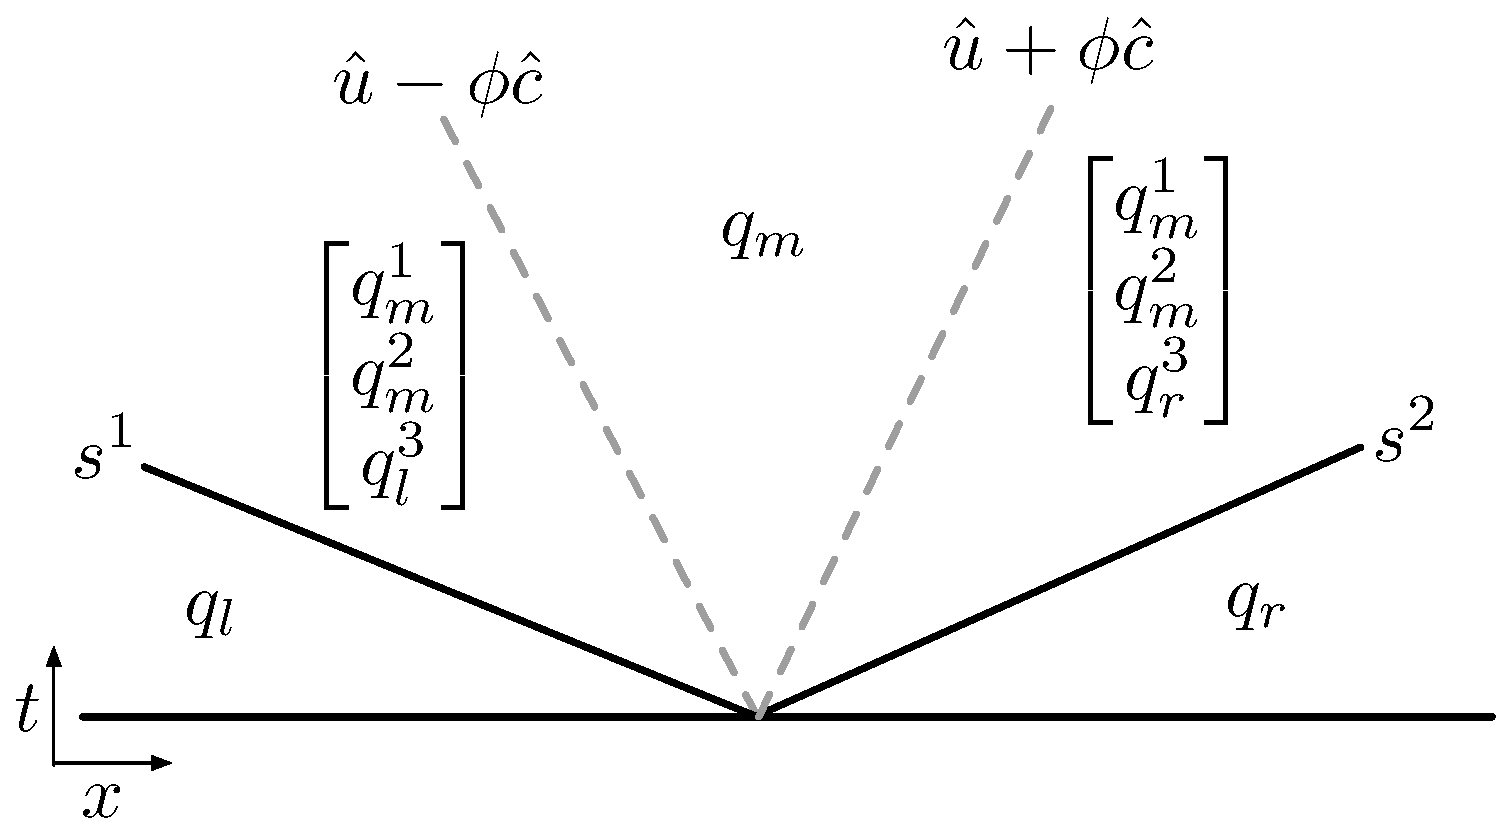
\includegraphics[width=0.6\textwidth]{figures/hllemcc.pdf}
    \caption{Structure of the HLLEMCC approximate Riemann solution, with four waves.}
    \label{HLLEMCC}
\end{figure}

\section{Entropy dissipative Riemann solver}\label{sec:ent_diss_rs}
Consider a hyperbolic system of conservation laws 
\begin{align}\label{cons_law}
  \frac{\partial \bfu(\bfx)}{\partial t} + \nabla\cdot \bff(\bfu(\bfx))=0, \quad \bfx\in\Omega,
\end{align}
with a en entropy pair $\left(\eta(\bfu), \bfq(\bfu)\right)$. 
A weak solution of \eqref{cons_law} is called an entropy solution if 
\begin{align}\label{ent_inequality}
  \frac{\partial \eta(\bfu(\bfx))}{\partial t} + \nabla\cdot \bfq(\bfu(\bfx))\leq 0, \quad \bfx\in\Omega,
\end{align}
holds, in a distribution sense, for any entropy pair.
It is desirable for a numerical method to satisfy a discrete version of the entropy inequality 
\eqref{ent_inequality}. This is, however, not true for many standard numerical discretizations. 
In general, an entropy stable scheme introduces nonlinear stabilization, which is 
particularly important for solutions with strong discontinuities that might converge to non-physical 
weak solutions. 
In this work, we propose an entropy stable approximate Riemann solver for the one dimensional 
shallow water equations. We use this Riemann solver as building block within the Lax-Wendroff-LeVeque 
method, as described in \cite{leveque1997wave,leveque2002finite} and implemented in Clawpack.

\subsection{Entropy residual}
Let $S_i$ be the set of cells containing cell $i$ and those that share a face with it. 
Also let $\bfv(\bfu)=\eta^\prime(\bfu)$ be the entropy variable. 
Based on \cite{guermond2011entropy}, we consider 
\begin{align}\label{ent_residual}
  \int_{S_i} \bfv(\bfu) \cdot \left[ \frac{\partial \bfu}{\partial t} + \nabla\cdot \bff(\bfu)\right]d\bfx
  =\int_{S_i} \left[\frac{\partial \eta(\bfu)}{\partial t} + \bfv(\bfu) \cdot \nabla\cdot \bff(\bfu)\right] d\bfx
\end{align}
as a measurement of the entropy production in $S_i$. 
To avoid approximating the time derivative of the entropy, we follow 
\cite{guermond2018second, guermond2018well} and use 
$\int_{K_i} \frac{\partial\eta(\bfu)}{\partial t}d\bfx=-\int_{K_i} \nabla\cdot\bfq(\bfu) d\bfx$, 
which holds in smooth regions. Then we define 
\begin{align}\label{Ri}
  R_i := \frac{N_i}{D_i}, 
\end{align}
with
\begin{align*}
  N_i=
  \left|\int_{S_i} \left[\bfv(\bfu) \cdot \nabla\cdot \bff(\bfu) - \nabla\cdot\bfq(\bfu) \right] d\bfx\right|,
\end{align*}
and $D_i$ being an upper bound of $N_i$ that acts as normalization so that $0\leq R_i\leq 1$.
Note that $N_i\approx 0$ if $\bfu$ is smooth in $S_i$. 
In our implementation, we use
\begin{align*}
  N_i\approx \left|\bfv(\bfu_i)\cdot \int_{S_i}\nabla\cdot \bff(\bfu)d\bfx 
  -\int_{S_i}\nabla\cdot\bfq(\bfu) d\bfx\right|,
  \quad 
  %D_i = ||\bfv(\bfu_i)||_{\ell^2}\left|\left|\int_{S_i}\nabla\cdot\bff(\bfu)d\bfx\right|\right|_{\ell^2}
  %+\left|\int_{S_i}\nabla\cdot\bfq(\bfu)d\bfx\right|.
  D_i = \sum_{k=1}^{d+1}|\bfv_k(\bfu_i)|\left|\int_{S_i}\left(\nabla\cdot\bff(\bfu)\right)_kd\bfx\right|
  +\left|\int_{S_i}\nabla\cdot\bfq(\bfu)d\bfx\right|,
\end{align*}
where $({\bf z})_k$ denotes the $k$-th component of ${\bf z}\in\mathbb{R}^{d+1}$ and $d$ is the number of physical 
dimensions. In the next section, we use $R_i$ to blend Rusanov's and Roe's Riemann solvers. 

\subsection{Blended Riemann solver}\label{sec:blended_rs}
In this section, we use \eqref{Ri}, which is a normalized measurement of the entropy residual \eqref{ent_residual}, 
to blend the Rusanov's and the Roe's Riemann solvers. To do this, we define the following numerical flux:
\begin{align}\label{num_flux_ev}
  F_{i+1/2} = \frac{\bff(\bfu_{i+1})+\bff(\bfu_i)}{2} 
  - \frac{1}{2} \left( R_{i+1/2}\lambda_{i+1/2}^{\max}\mathbb{I} + (1-R_{i+1/2})|\hat A_{i+1/2}| \right)(\bfu_{i+1}-\bfu_{i}),
\end{align}
and similarly for $F_{i-1/2}$. Here $\mathbb{I}\in\mathbb{R}^{3\times 3}$ is the identity matrix,
$R_{i+1/2}=\max\{R_{i+1},R_i\}$, $\lambda_{i+1/2}^{\max}$ is the 
upper bound on the wave speed used in the Rusanov's Riemann solver, see \S \ref{sec:rusanov}, 
and $\hat A_{i+1/2}$ is the Roe's averaged flux Jacobian, see \S \ref{sec:roe}. 

%In terms of fluctuations, 
The first-order method is given simply by \eqref{first-order_FV} 
with the numerical flux $F_{i+1/2}$ given by \eqref{num_flux_ev}. 
In smooth regions $R_{i+1/2}\approx 0$ so the numerical flux is essentially the Roe's numerical flux. 
Near discontinuities or steep gradients, $R_{i+1/2}$ becomes large. If, in particular, $R_{i+1/2}\approx 1$, 
then the numerical flux is essentially the Rusanov's numerical flux.  
%
The first-order method can also be written in terms of fluctuations via \eqref{first-order_via_fluct}. 
To do this we consider the waves ($\W^p_{i\pm 1/2}$, with $p=1,2,3$) 
from the Roe's solver and define 
\begin{align}\label{lambda_p}
  \lambda_{i+1/2}^p := R_{i+1/2}\lambda_{i+1/2}^{\max} + (1-R_{i+1/2})|\hat \lambda_{i+1/2}^p|,
\end{align}
where $\hat\lambda_{i+1/2}^p$ is the $p$-th eigenvalue of the Roe's solver corresponding to the 
interface $i+1/2$. Note that $\lambda_{i+1/2}^p\geq 0$.
The fluctuations are then given by 
\begin{subequations}\label{ev_fluctuations}
\begin{align}
  \A^+\Delta Q_{i-1/2}&=\frac{1}{2}\sum_p \left(\hat\lambda_{i-1/2}^p + \lambda_{i-1/2}^p\right)\W_{i-1/2}^p, \\
  \A^-\Delta Q_{i+1/2}&=\frac{1}{2}\sum_p \left(\hat\lambda_{i+1/2}^p - \lambda_{i+1/2}^p\right)\W_{i+1/2}^p.
\end{align}
\end{subequations}

To implement the second-order Lax-Wendroff-LeVeque type method in Clawpack, the Riemann solver must provide 
the fluctuations, the waves and their speed. The fluctuations are simply \eqref{ev_fluctuations} 
and the waves are the Roe's waves $\W_{i+1/2}^p$, with $p=1,2,3$. 
In the framework of LeVeque, for a given interface $i+1/2$, 
we would need to consider a wave speed $s_{i+1/2}^p$ so that 
\begin{align*}
  \hat \lambda_{i+1/2}^p+\lambda_{i+1/2}^p = s_{i+1/2}^p+|s_{i+1/2}^p|, \qquad 
  \hat \lambda_{i+1/2}^p-\lambda_{i+1/2}^p = s_{i+1/2}^p-|s_{i+1/2}^p|,
\end{align*}
which is not possible to obtain in general (since the problem is overdetermined). 
Instead, we consider 
$s_{i+1/2}^p=\sgn(\hat\lambda_{i+1/2}^p)\lambda_{i+1/2}^p$ 
 and study the consequences of this choice once the second-order corrections are applied.
Here $\sgn(z)$ is the sign function of $z$. 
The second-order Lax-Wendroff-LeVeque method for the one-dimensional problem is given by 
\begin{align}\label{second-order}
  u_i^{n+1}=u_i^n
  -\frac{\Delta t}{\Delta x}\left[\A^-\Delta Q_{i+1/2}+\A^+\Delta Q_{i-1/2}\right]
  -\frac{\Delta t}{\Delta x}\left[\tilde F_{i+1/2}-\tilde F_{i-1/2}\right],
\end{align}
where 
\begin{align*}
  \tilde F_{i+1/2} = \frac{1}{2}\sum_p\lambda_{i+1/2}^p
  \left(1-\frac{\Delta t}{\Delta x}\lambda_{i+1/2}^p\right)\tilde\W_{i+1/2}^p,
\end{align*}
and similarly for $\tilde F_{i-1/2}$, are the flux corrections with $\tilde\W_{i+1/2}^p$ 
being a TVD-limited version of $\W_{i+1/2}^p$. 

To understand the effect of choosing $s_{i+1/2}^p=\sgn(\hat\lambda_{i+1/2}^p)\lambda_{i+1/2}^p$ 
as the speed of $\W_{i+1/2}^p$, 
let us assume that no limiters are applied; i.e., $\tilde\W_{i\pm 1/2}^p\equiv \W_{i\pm 1/2}^p$.
By doing this, equation \eqref{second-order} can be written as 
\begin{align*}
  u_i^{n+1}=u_i^n
  &-\frac{\Delta t}{2 \Delta x}
  \sum_p
  \left[\left(\hat\lambda_{i+1/2}^p -\frac{\Delta t}{\Delta x}(\lambda_{i+1/2}^p)^2 \right)\W_{i+1/2}^p
  +
  \left(\hat\lambda_{i-1/2}^p +\frac{\Delta t}{\Delta x}(\lambda_{i-1/2}^p)^2 \right)\W_{i-1/2}^p\right],
\end{align*}
which corresponds to the standard Lax-Wendroff method written in terms of fluctuation-like quantities. 
Note that if $R_{i\pm 1/2}=0$, we recover the standard second-order Lax-Wendroff method based on 
Roe's Riemann solver. 
In the numerical experiments in \S\ref{sec:num}, we obtain second-order experimental 
order of convergence (EOC) for problems with smooth solution, which is expected since 
$R_{i\pm 1/2}\approx 0$ in smooth regions.
Similarly, if $R_{i\pm 1/2}=1$, we recover the Lax-Wendroff method based on Rusanov's Riemann solver, 
which is clear by writting the fluctuations in Rusanov's method in terms of Roe's waves and speeds, 
see \eqref{fluct_rus}.


\subsection{Entropy stable Riemann solver}
The Riemann solver presented in the previous section blends Rusanov's and Roe's solver based on a
measurement of the entropy residual. The objective is to induce dissipation of entropy 
near discontinuities. However, we have no guarantee that methods \eqref{first-order_via_fluct} 
or \eqref{second-order_via_fluct} based on this Riemann solver are (locally) entropy stable. 
In this section, we consider the one-dimensional problem and increase the numerical dissipation 
to guarantee entropy stability for \eqref{first-order_via_fluct}. 
To this end we follow the work by Tadmor, see for instance \cite{tadmor1987numerical, tadmor2003entropy} 
and references therein. 

Recall method \eqref{first-order_FV}
\begin{align*}
  \bfu_i^{n+1}=\bfu_i^n-\frac{\Delta t}{\Delta x}\left[\bfF_{i+1/2}-\bfF_{i-1/2}\right],
\end{align*}
with the numerical fluxes given by 
\begin{align*}
  \bfF_{i+1/2} = \frac{\bff(\bfu_{i+1})+\bff(\bfu_i)}{2} 
  - \frac{1}{2} \left( R_{i+1/2}\lambda_{i+1/2}^{\max}\mathbb{I} + (1-R_{i+1/2})|\hat A_{i+1/2}| +\lambda_{i+1/2}^{\min}\mathbb{I}\right)(\bfu_{i+1}-\bfu_{i}),
\end{align*}
and similarly for $\bfF_{i-1/2}$. Here $\lambda_{i+1/2}^{\min}$ is yet to be defined.
We can write the numerical fluxes in terms of $\lambda^p_{i\pm 1/2}$ \eqref{lambda_p}
and the Roe's waves $\W_{i\pm 1/2}^p$.
Doing so, we get
\begin{align*}
  \bfF_{i+1/2} = \frac{\bff(\bfu_{i+1})+\bff(\bfu_i)}{2} 
  - \frac{1}{2}\sum_p(\lambda_{i+1/2}^p+\lambda_{i+1/2}^{\min})\W_{i+1/2}^p,
\end{align*}
and similarly for $\bfF_{i-1/2}$.
Let $\bfv_i=\bfv(\bfu_i)$ and $q_i=q(\bfu_i)$ denote the entropy variable and the 
(one-dimensional) entropy potential at cell $i$, respectively. 
Also let $\psi_i=\bfv(\bfu_i)\cdot \bff(\bfu_i)-q(\bfu_i)$ be the entropy potential at cell $i$.
From \cite[\S 4]{tadmor1987numerical}, if the numerical fluxes satisfy
\begin{align}\label{es_cond}
(\bfv_{i}-\bfv_{i-1})\cdot \bfF_{i-1/2}\leq \psi_{i}-\psi_{i-1},
  \qquad
  (\bfv_{i+1}-\bfv_i)\cdot \bfF_{i+1/2}\leq \psi_{i+1}-\psi_i,
\end{align}
then the following entropy inequality holds 
\begin{align}\label{ent_ineq}
  \frac{d\eta(\bfu_i)}{dt}+\frac{1}{\Delta x}\left[G_{i+1/2}-G_{i-1/2}\right]\leq 0,
\end{align}
where 
\begin{align*}
    G_{i+1/2} &= \frac{1}{2}\left(\bfv_i+\bfv_{i+1}\right)\bfF_{i+1/2}-\frac{1}{2}(\psi_{i}+\psi_{i+1}),
\end{align*}
and similarly for $G_{i-1/2}$, are discretizations of the entropy flux. 

Based on \eqref{es_cond}, we choose
\begin{align}\label{lambda_min}
  \lambda_{i+1/2}^{\min} = \max\left\{0,\frac{\frac{1}{2}(\bfv_{i+1}-\bfv_{i})\cdot\left[\bff(\bfu_{i+1})+\bff(\bfu_{i})-\sum_p\lambda_{i+1/2}^p\W_{i+1/2}^p\right]-(\psi_{i+1}-\psi_i)}{\frac{1}{2}(\bfv_{i+1}-\bfv_{i})\cdot\sum_p\W_{i+1/2}^p}\right\}
\end{align}
which guarantees \eqref{es_cond} and, therefore, \eqref{ent_ineq}. 
Since the blended Riemann solver induces dissipation of entropy, 
we expect condition \eqref{es_cond} to be fulfilled most of the times even with $\lambda_{i+1/2}^{\min}=0$. 
Therefore, \eqref{lambda_min} is used as a safeguard to guarantee entropy stability
for the one-dimensional problem using method \eqref{first-order_FV} or \eqref{first-order_via_fluct}. 
Extra modifications are needed to guarantee entropy stability of Lax-Wendroff-LeVeque method 
\eqref{second-order_via_fluct} and its multidimensional extension via Strang's splitting. 
We do not pursue these modifications in this work. 

\begin{remark}
In terms of fluctuations, the entropy stability condition \eqref{es_cond} can be written as 
\begin{align*}
  (\bfv_{i}-\bfv_{i-1})\cdot 
  \Big(
  \underbrace{\bff(\bfu_i)-\A^+\Delta Q_{i-1/2}}_{=\bfF_{i-1/2}}\Big)\leq \psi_{i}-\psi_{i-1},
  \quad
  (\bfv_{i+1}-\bfv_i)\cdot 
  \Big(\underbrace{\bff(\bfu_i)+\A^-\Delta Q_{i+1/2}}_{=\bfF_{i+1/2}}\Big)\leq \psi_{i+1}-\psi_i.
\end{align*}
\end{remark}



\clearpage
\section{Numerical results}\label{sec:num}
Description of the methods. We consider either the first-order method XX or the second-order Lax-Wendroff
type method XX. For each of these methods we use one of the following three Riemann solvers: 
\begin{itemize}
  \item LLF: Rusanov's or Local Lax Friederichs 2-wave Riemann solver reviewed in \S XX.
  \item Roe: standard Roe's average based 3-wave Riemann solver reviewed in \S XX. 
  \item Roe-fix: Roe's solver with entropy fix based on XX. 
  \item EV:  entropy dissipative 3-wave Riemann solver described in \S XX.
\end{itemize}

\subsection{Dam break problem on a dry bed}
We start with the one-dimensional dam break problem on a dry bed. 
This problem is a canonical example that demonstrates the `entropy glitch' of Roe's solver 
at transonic rarefactions. Since the baseline Roe's solver we use (see \S XX) does not contain 
an entropy fix, it is important to demonstrate that the blended Riemann solver fixes the entropy glitch, 
at least for this benchmark. 
We follow the setup in XX. The domain is given by XX, and the initial condition is XX and XX. 
The exact solution, which can be found in XX and references therein, is 

XX 

We use g=1 and solve the problem up to T=10. In Figure XX we show the solution using method XX 
with Roe's solver, Rusanov's solver and the blended solver. The entropy glitch, which is manifested 
as a non-physical show at x=XX, is clearly shown with Roe's solver. Using Rusanov's solver and the 
blended solver fix the entropy glitch. Using the blended solver leads to more accurate results. 
In Table XX, we summarize the results of a convergence test. 

\subsection{Dam break problem on a wet bed}
We consider a one-dimensional dam break problem on a wet domain. 
We follow the setup in XX. 
The domain is $\Omega=(0,L)$ with $L=10$, the initial condition is given by 
$hu(x,0)=0$ and 
\begin{align*}
  h(x,0) = 
  \begin{cases}
    h_l & \mbox{ if } x\in(0,x_0], \\
    h_r & \mbox{ if } x\in(x_0,L),
  \end{cases}
\end{align*}
with $x_0=5$, $h_l=0.005$ and $h_r=0.001$. 
The exact solution, which can be found in XX and references therein, is given by 
\begin{align*}
  h(x,t) = 
  \begin{cases}
    h_l, \\
    \frac{4}{9g}\left(\sqrt{gh_l}-\frac{x-x_0}{2t}\right)^2, \\
    \frac{c_m^2}{g}, \\
    h_r, 
  \end{cases}
\quad 
  u(x,t) = 
  \begin{cases}
    0, &\mbox{ if } x\leq x_A(t), \\
    \frac{2}{3}\left(\sqrt{gh_l}+\frac{x-x_0}{t}\right), & \mbox{ if } x_A(t) < x\leq x_B(t), \\
    2(\sqrt{gh_l}-c_m), & \mbox{ if } x_B(t)<x\leq x_C(t), \\
    0, &\mbox{ if } x\leq x_C(t),
  \end{cases}
\end{align*}
where $x_A(t)=x_0-t\sqrt{gh_l}$, $x_B(t)=x_0+t\left(2\sqrt{gh_l}-3c_m\right)$, 
$x_C(t)=x_0+t\frac{2c_m^2\left(\sqrt{gh_l}-c_m\right)}{c_m^2-gh_r}$ and 
$c_m$ is the solution of 
$-8gh_rc_m^2\left(\sqrt{gh_l}-c_m\right)^2+\left(c_m^2-gh_r\right)^2\left(c_m^2+gh_r\right)=0$.
We use $g=1$ and solve the problem up to the final time $T=5$ considering the 2nd-order Lax-Wendroff 
type method XX with the LLF, Roe and EV Riemann solvers. The solution with different refinement levels 
and each Riemann solver is shown in Figure XX. In Table XX, we summarize the results of a convergence test. 
Since the solution is non-smooth, we expect no more than first order convergence rates. Note that the 
results with the entropy dissipative solver EV are comparable against the results using Roe's solver. 
That is, inducing entropy dissipation via the EV Riemann solver does not degrade the high-order accuracy 
properties of the Roe's solver. 
In contrast, the accuracy and convergence rates using the LLF solver are clearly degraded.  

\subsection{The circular hydraulic jump in one dimension}

\subsection{Steady outflow}
Let us consider a problem similar to that in the previous section, but with an outflow boundary condition. 
That is, we consider the one-dimensional domain $\Omega=(0.1,1)$, the initial condition is 
$h(x,t=0)=0.1$, $hu(x,t=0)=0$, the left boundary condition is $h(0.1,t)=0.3$, $hu(0.1,t)=0.75$, 
and the right boundary condition is set to outflow, see the details in XX. 
If the flow is supercritical ($|F|>1$), the exact solution converges to a 
steady state profile given by the solution of the ODE XX. 
Depending on the initial condition, shocks might develop before the steady state is reached. 
Nevertheless, the steady state profile is smooth. 
In Figure XX, we show the solution at different times based on the secnd-order method XX with 
the EV Riemann solver. Additionally, in Table XX we summarize the result of a convergence study 
based on the first- and second-order methods XX and XX, respectively. 
We consider the Riemann solver in \S XX with Ri=0, Ri=1 and Ri computed via XX. 


\subsection{The circular hydraulic jump in two dimensions}
We consider two regimes. In the first regime, the physical instabilities are mild. 
By increasing the strength of the jump and other parameters, we consider a second 
and more strongly unstable regime. In both cases, we generate the CHJ as described in 
Section XX; that is, we impose supersonic inflow boundary conditions for the jet and 
subsonic outflow boundary conditions. 

We consider two types of domain and two corresponding computational grids. 
The two types of domains are two-dimensional squares and circular domains. 
For both cases we use structured grids. See an example of these domains and grids in Figures XX and XX, 
respectively.

\subsection{Regime 1: midly unstable flow}

Show the results with Roe's and Rusanov's solver. 
Show the results with the three proposed methodologies. 

\subsection{Regime 2: strongly unstable flow}

Show the results with Roe's and Rusanov's solver. 
Show the results with the three proposed methodologies. 

\section{Conclusions}

\appendix
\section{Bow shock problem for the shallow water equations}

\section{Other numerical studies}

%\bibliographystyle{apalike}
\bibliographystyle{plain}
\bibliography{refs}

\end{document}

%Random perturbation only in the jet
%Turn off the perturbation after some time
%Reduce the amplitude of the perturbation 
%Non-rotationally sym. IC 
%Consider Kemm's solver. 


